\subsubsection{Downstream Processing}
\index{Fernandez-Lahore, Marcelo}


\paragraph{Research Team}
%
Marcelo Fernandez-Lahore (Professor), Sabine Binner (Technical Assistant), Rosa Cabrera (Postdoc), Rami Reddy Vennapusa (PhD Student), Farnoosh Dairpoosh (PhD Student), Leonardo Galvis (Graduate Student), Rustem Khusainov (Graduate Student)\\


Our work at Jacobs University has the main goal of the meta-integration between
the various bioproduct purification strategies that have been described
 previously in an isolate manner. The prefix meta- is thus
 ``used with the name of a discipline to designate a new but
  related discipline designed to deal critically with the original one''
  (Webster Dictionary). Up to now, no general rules exist on how to
   combine in the more efficient way process technology, combinatorial
   techniques, and genetic engineering tools. We are exploring this situation
    utilising a number of relevant industrial (bio) products. From the knowledge generated within the frame of our project(s) it is expected that general recommendations to guide industrialists will emerge. Clearly, this will translate in facilitated bioprocessing.

\paragraph{Highlights}
%
We have developed a novel Definitive Bioseparation Engineering concept based on mass screening experiments to exactly define de nature of the ``purification proteome'' for the chosen product expression system. ``Proteome spaces'' where proteins from the expression system are minimized or inexistent are being identified. Directing the targeted product to the same will allow attaining $-$or at least to very closely approaching$-$ the ``one-binding species'' situation. We have already shown that under these conditions prediction of large-scale processes is possible on the basis of simple analytical equations. Changing the relative ``proteome coordinates'' between product and contaminants will be attempted by introduction of protein tags or via dedicated ligand chemistry. Evidence-based results from scouting experiments will be compared to the expected binding of MS/MS identified host proteins to immobilized functional adsorbent groups. Emphasis will be on understanding the influence of the
 chemical environment provided by the solid phase, coupling chemistry and nature of the ligand in relation with protein surface.


\begin{figure}[ht]
  \begin{center}
   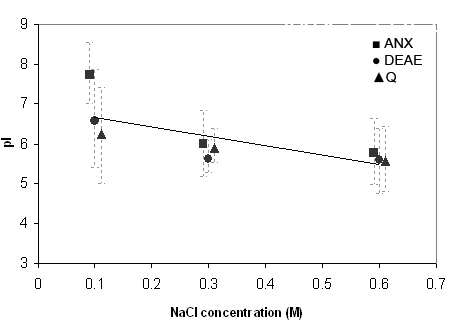
\includegraphics[width=\hsize]{Fernandez-Lahore/Fernandez-Lahore_new.png}
    \mycaption{Mean \& SD of isoelectric point values among the observed spots and the relationship between these values and the NaCl concentration of the corresponding material.}\label{fig2:Lahore}
     \end{center}
\end{figure}

%Achtung
Cell disruption constitutes and essential processing step for yeast
intracellular products, which is known to influence the quality of
fluidization and the sorption performance in `expanded' bed systems.
Cell electro-permeabilization coupled to direct product sorption on
expanded beds contactors was explored. S. cerevisiae F17 was pulsated in
batch mode (10 pulses, 1.5 ms, 4kV/cm, 2 Hz) and the properties of the
resulting cell particles studied via surface thermodynamic approaches.
Several process-relevant observations were made: a) The enzyme utilized
as model glyceraldehyde-3-phosphate dehydrogenase, GAPDH- was
released with high yield (87\%) and good purification factor (1.5-2.0)
in comparison with cell lysate as control; b) A shift in the surface
properties of the cell particles was noticed e.g., the Z-potential
changed from -12 mV to -9 mV upon pulsation while AB (-55 mN/m) and LW
(+30 mN/m) components suffered only minor change
at pH 7; c) A reduced interaction of the electroextracted feedstock with
DEAE-Streamline adsorbents was evidenced by the biomass pulse method
i.e. cell transmission increased from 14\% to 41\% after pulsation; and
d) the model product was purified by direct contact with a global yield
of 59-76\% and purification factor of 12. Moreover, low protease
activity was also observed i.e., 20\% of the activity present in the
mechanically disrupted cell paste.
A novel primary recovery route for yeast intracellular bioproducts can
be proposed by combination of selective permeabilization and immediate
sequestration on a solid phase. This will translate in increased product
quality, process yield, and cost-effectiveness.


%Cell disruption constitutes and essential processing step for yeast intracellular products, which is known to influence the quality of fluidization and the sorption performance in `expanded' bed systems.
%Cell electro-permeabilization coupled to direct product sorption on expanded beds contactors was explored. S. cerevisiae F17 was pulsated in batch mode (10 pulses, 1.5 ms, 4kV/cm, 2 Hz) and the properties of the resulting cell particles studied via surface thermodynamic approaches.
%Several process-relevant observations were made: a) The enzyme utilized as model $-$glyceraldehyde-3-phosphate dehydrogenase, GAPDH- was released with high yield (87\%) and good purification factor (1.5-2.0) in comparison with cell lysate as control; b) A shift in the surface properties of the cell particles was noticed e.g., the Z-potential changed from $-$12 mV to $-$9 mV upon pulsation while AB (?+ 3-4 mN/m, ?- 51-55 mN/m) and LW (28-30 mN/m) components suffered only minor change at pH 7; c) A reduced interaction of the electroextracted feedstock with DEAE-Streamline adsorbents was evidenced by the biomass pulse method i.e. cell transmission increased from 14\% to 41\% after pulsation; and d) the model product was purified by direct contact with a global yield of 59-76\% and purification factor of ?12. Moreover, low protease activity was also observed i.e., ? 20\% of the activity present in the mechanically disrupted cell paste.
%A novel primary recovery route for yeast intracellular bioproducts can be proposed by combination of selective permeabilization and immediate sequestration on a solid phase. This will translate in increased product quality, process yield, and cost-effectiveness.


\myparagraph{Collaborations}
National \& International Collaborations:
\begin{enumerate}
\item {\sl National University of Quilmes (Buenos Aires)} \\ Prof.  M. Grasselli \\ Novel materials for downstream processing of bioproducts
\item {\sl Pablo Cassara Foundation (Buenos Aires)}  Dr. M.A. Alvarez \\ Molecular Pharming
\end{enumerate}


\nocite{Fernandez-Lahore1,Fernandez-Lahore2,Fernandez-Lahore3,Fernandez-Lahore4,Fernandez-Lahore5,Fernandez-Lahore6,Fernandez-Lahore7}